% All figure environments (journal). Each figure is a macro that is called once, next to the text that first discusses it.
% Conference version: figs_conf.tex.
\newcommand{\figArch}{\begin{figure}[htbp]
\centering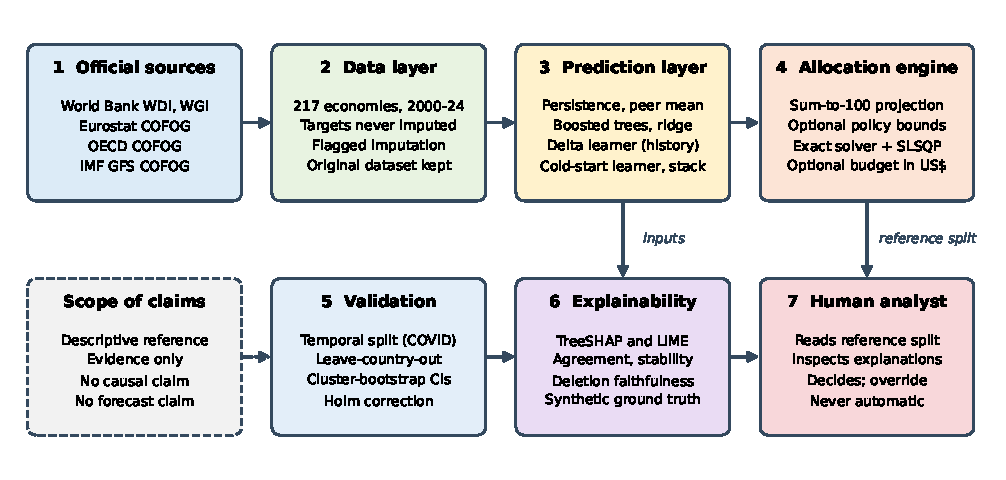
\includegraphics[width=\textwidth]{figures/fig1_architecture.pdf}
\caption{Evaluated components of GovAllocXAI. Official sources feed a flagged data layer; the prediction layer offers a history-based $\Delta$-learner and a cold-start peer learner; a bounded-simplex projection enforces the budget identity and optional bounds; explanations and a validation protocol surround every prediction; the intended user is a human analyst.}\label{fig:arch}
\end{figure}}
\newcommand{\figCoverage}{\begin{figure}[htbp]
\centering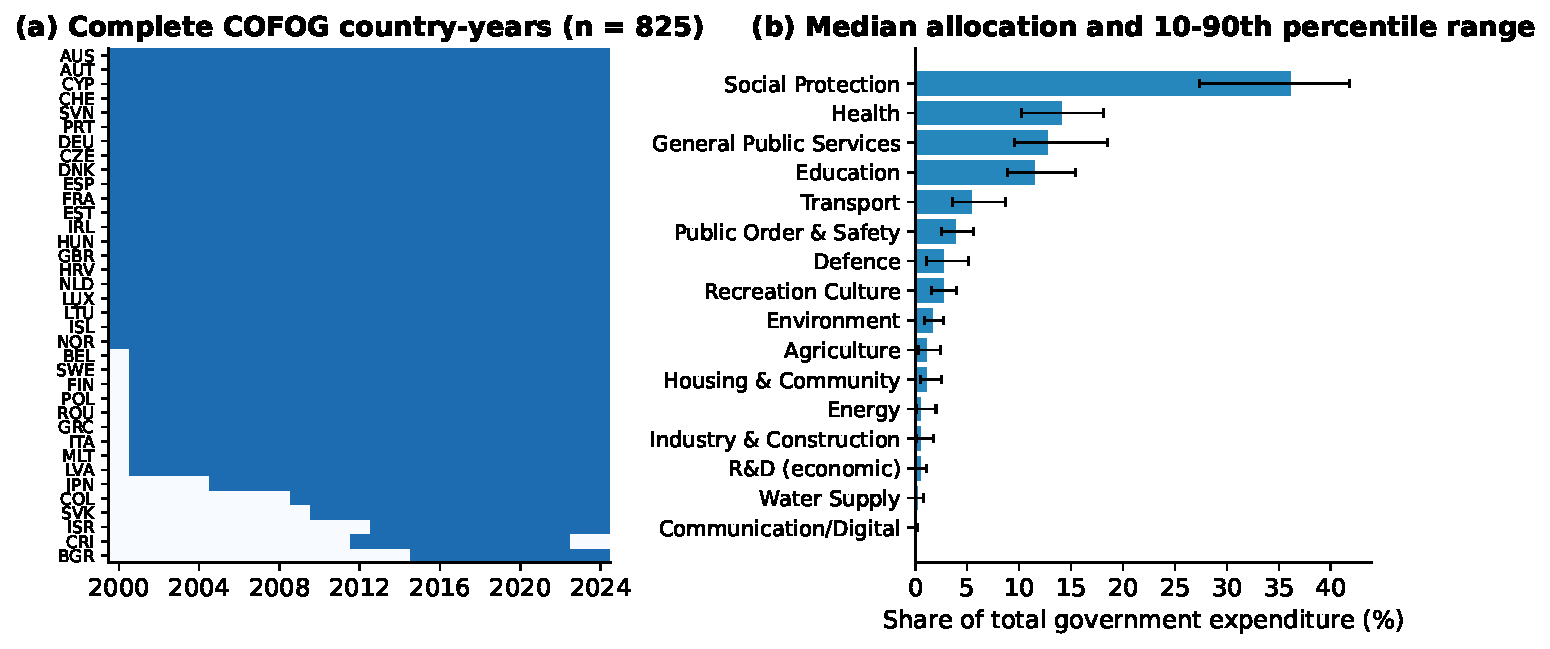
\includegraphics[width=\textwidth]{figures/fig2_data_coverage.pdf}
\caption{Data (panel A16). (a) Country-years with a complete 16-function COFOG breakdown (Eurostat for EU/EFTA, OECD otherwise). (b) Median share of total government expenditure per function with 10th--90th percentile range.}\label{fig:coverage}
\end{figure}}
\newcommand{\figAudit}{\begin{figure}[htbp]
\centering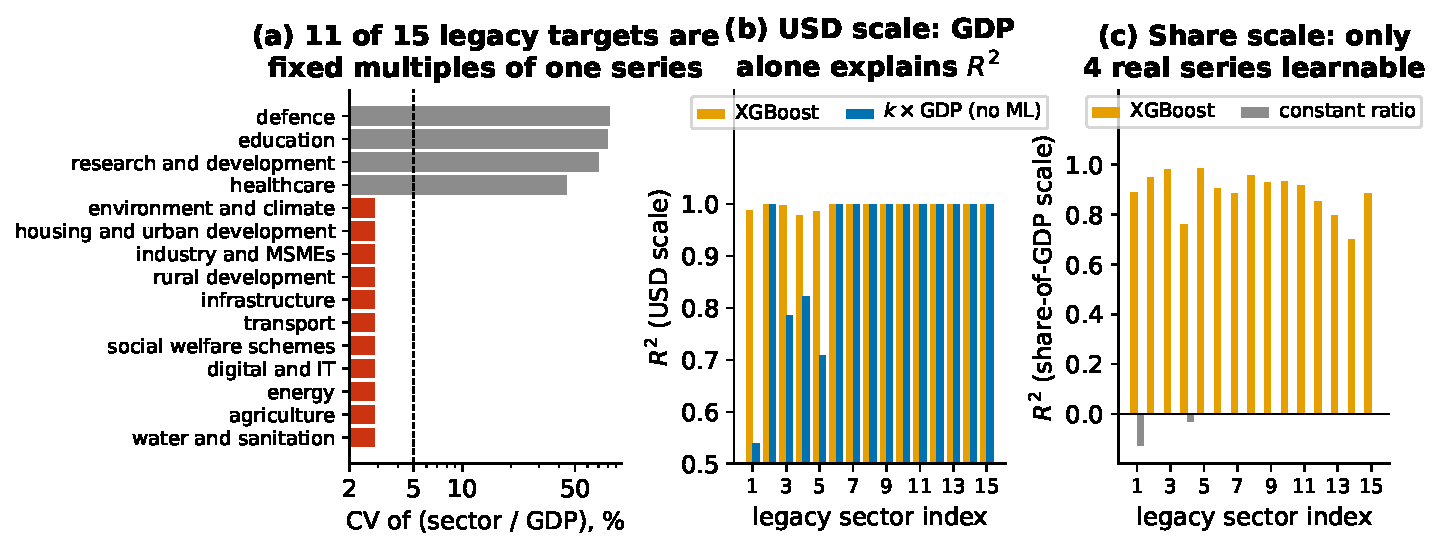
\includegraphics[width=\textwidth]{figures/fig3_legacy_audit.pdf}
\caption{Forensic audit of the legacy v1 benchmark ($n=775$ rows). (a) Coefficient of variation of sector/GDP: eleven sectors are below 5\% (they are exact multiples of one series). (b) On the USD scale a rule $k\times$GDP matches XGBoost on those sectors. (c) On the share-of-GDP scale a constant predictor has $R^2\approx0$ on them. Sector indices follow Table~\ref{tab:audit}.}\label{fig:audit}
\end{figure}}
\newcommand{\figMain}{\begin{figure}[htbp]
\centering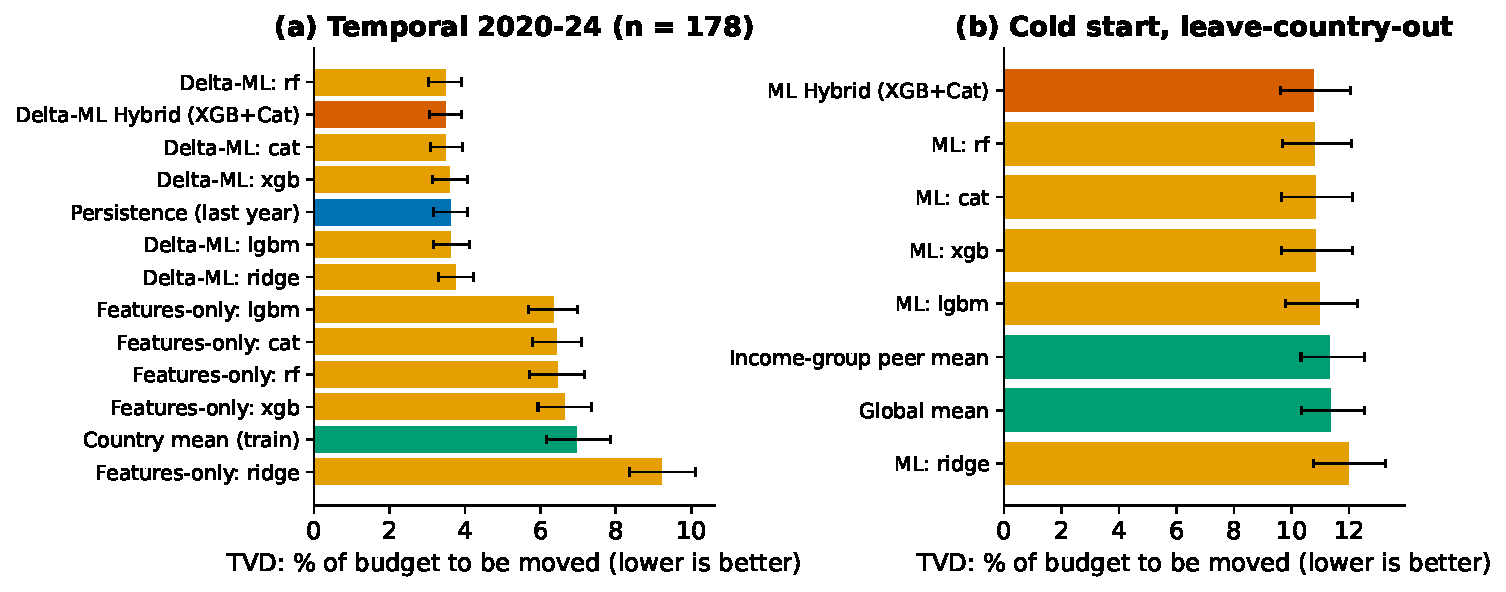
\includegraphics[width=\textwidth]{figures/fig4_main_results.pdf}
\caption{Main results on panel A16 (lower TVD is better; bars show 95\% cluster-bootstrap CIs). (a) Annual update, test 2020--24 ($n=178$): persistence is hard to beat. (b) Cold start, 825 country-years, two fold seeds: boosted learners vs.\ peer and global means.}\label{fig:main}
\end{figure}}
\newcommand{\figPerfn}{\begin{figure}[htbp]
\centering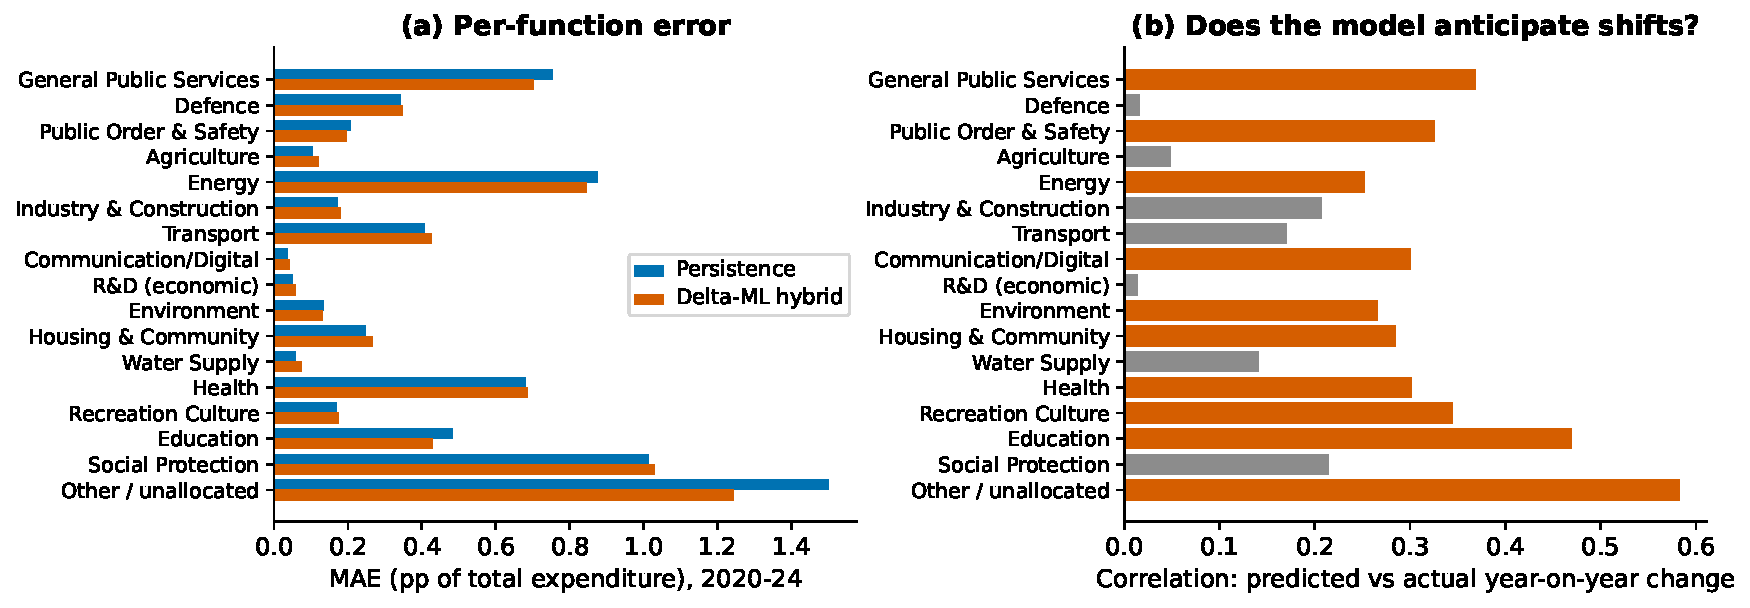
\includegraphics[width=\textwidth]{figures/fig5_per_function.pdf}
\caption{(a) Per-function error of persistence and the $\Delta$-hybrid on the 2020--2024 test window ($n=178$). (b) Correlation between predicted and observed year-on-year changes.}\label{fig:perfn}
\end{figure}}
\newcommand{\figWdi}{\begin{figure}[htbp]
\centering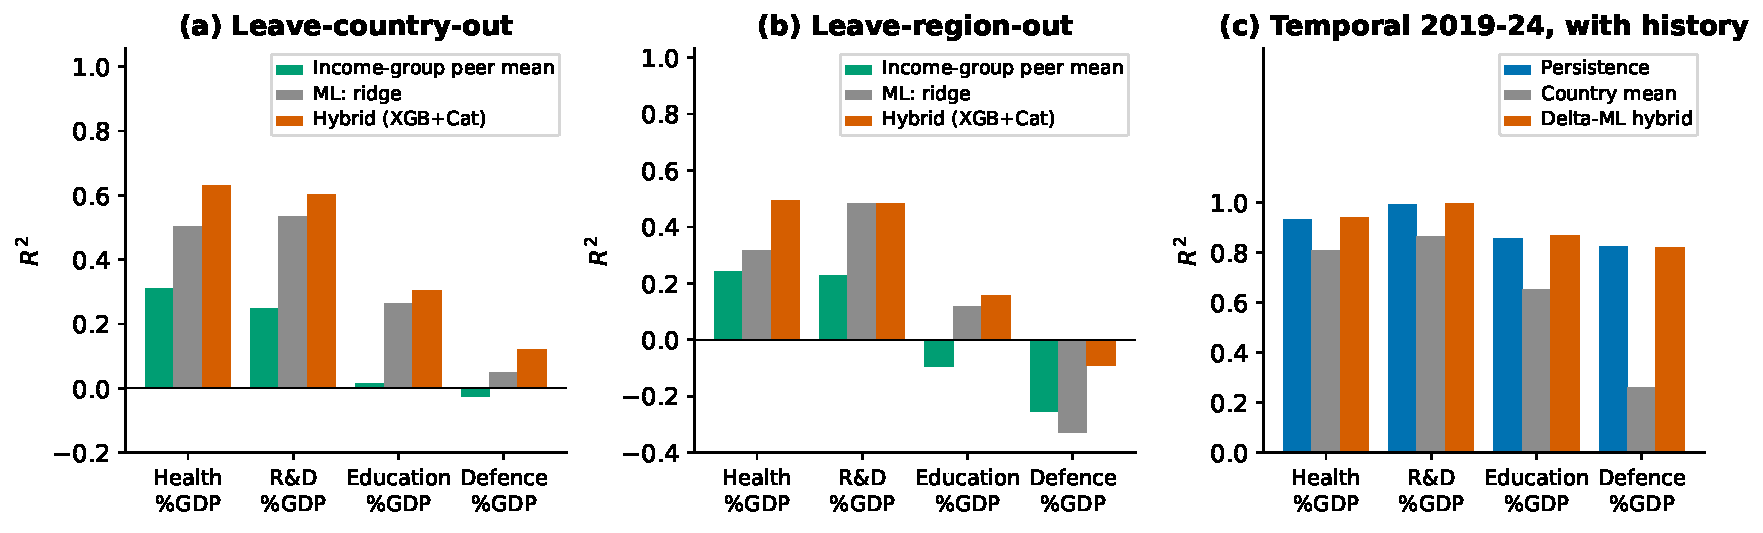
\includegraphics[width=\textwidth]{figures/fig6_wdi_panel.pdf}
\caption{Global WDI panel (one fold seed): $R^2$ for four official functions under (a) leave-country-out, (b) leave-region-out and (c) temporal evaluation.}\label{fig:wdi}
\end{figure}}
\newcommand{\figShap}{\begin{figure}[htbp]
\centering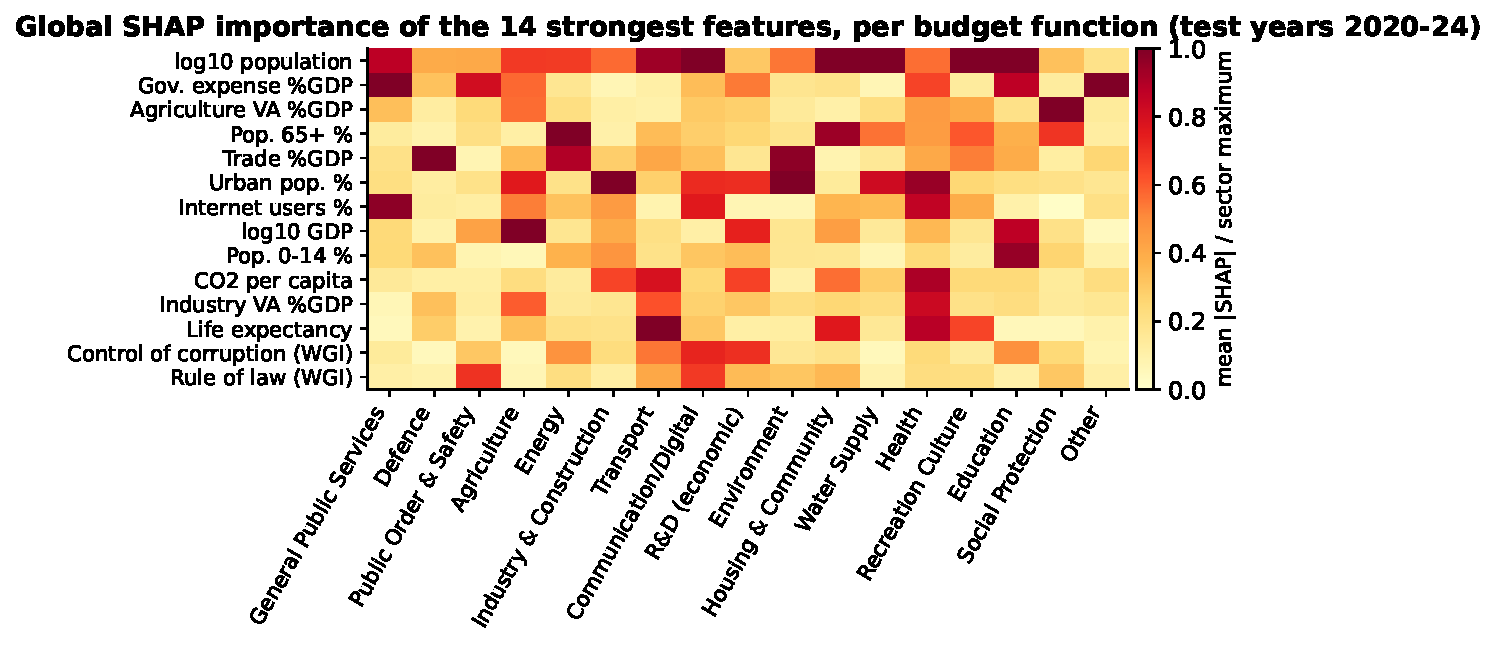
\includegraphics[width=0.9\textwidth]{figures/fig7_global_shap.pdf}
\caption{Global SHAP importance (mean $|\phi|$ normalised by each function's maximum) of the 14 strongest features for each budget function, test years 2020--24 (XGBoost member).}\label{fig:shap}
\end{figure}}
\newcommand{\figLime}{\begin{figure}[htbp]
\centering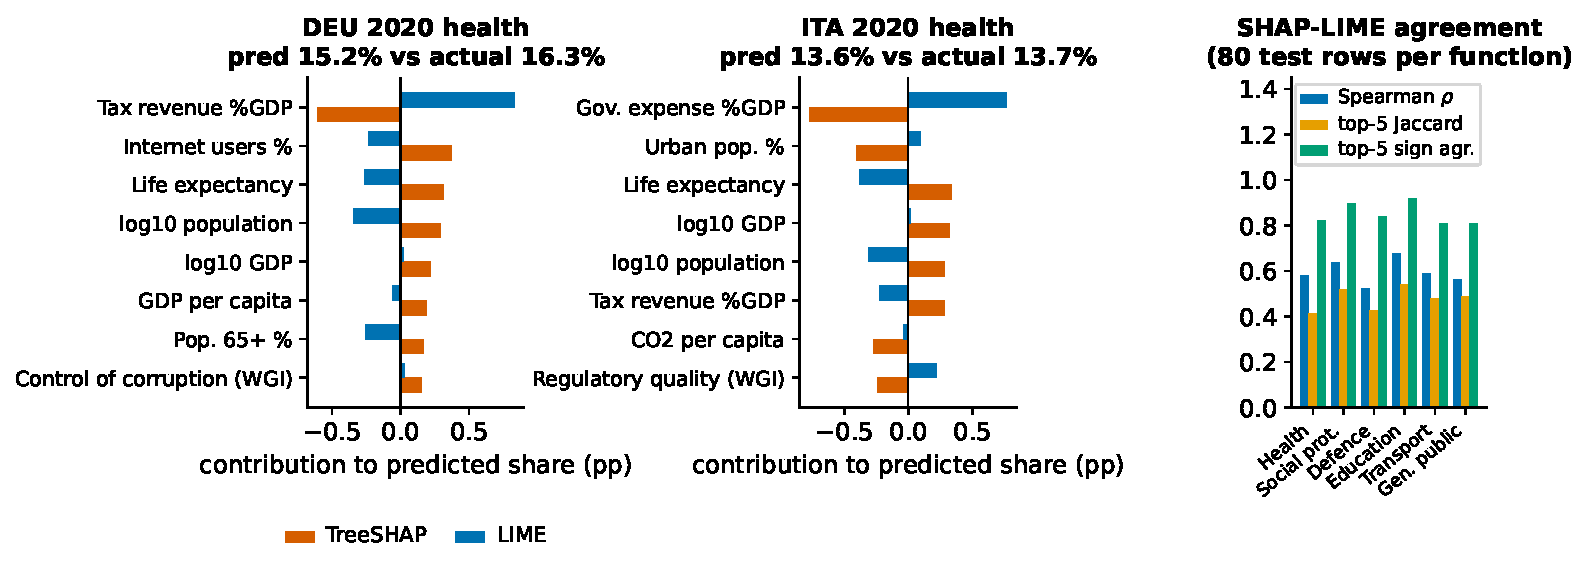
\includegraphics[width=\textwidth]{figures/fig8_shap_vs_lime.pdf}
\caption{SHAP vs.\ LIME. Left and centre: signed contributions for two test cases (feature values in Table~\ref{tab:features} units). Right: agreement metrics over 80 test rows per function.}\label{fig:lime}
\end{figure}}
\newcommand{\figWhatif}{\begin{figure}[htbp]
\centering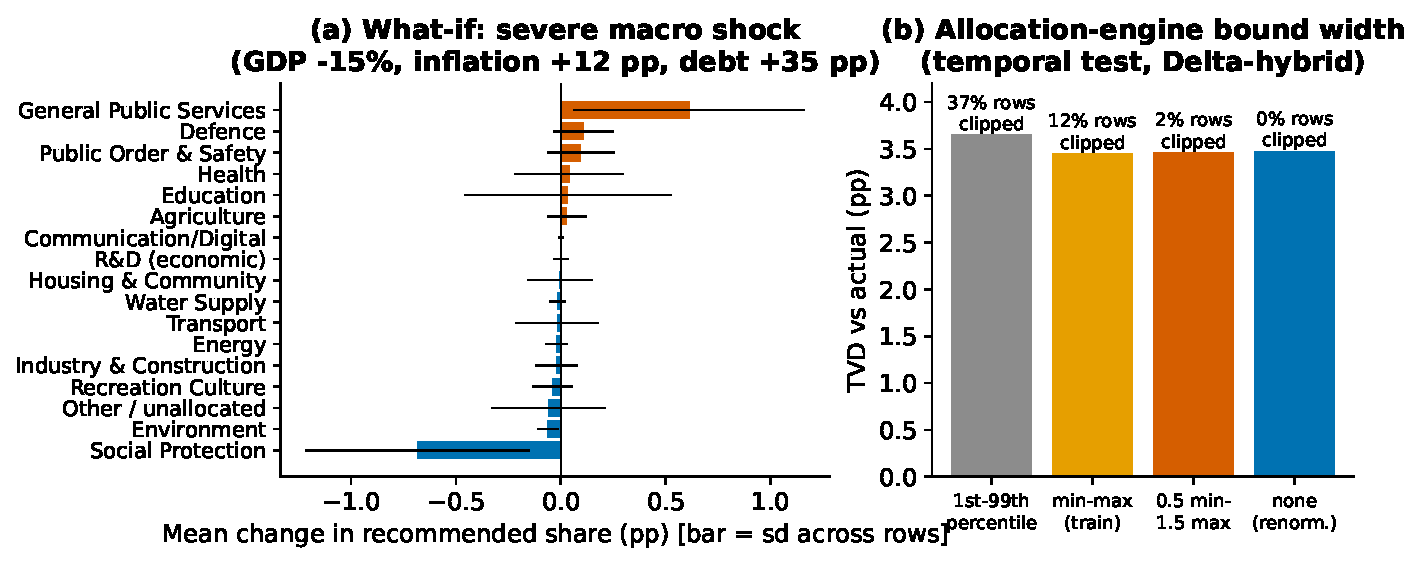
\includegraphics[width=\textwidth]{figures/fig9_whatif_engine.pdf}
\caption{(a) What-if sensitivity of the cold-start model to a severe macro shock (a model sensitivity, not a forecast). (b) Allocation-engine error vs.\ width of policy bounds (y-axis from zero); labels give the share of predictions that were clipped.}\label{fig:whatif}
\end{figure}}
\newcommand{\figCovid}{\begin{figure}[htbp]
\centering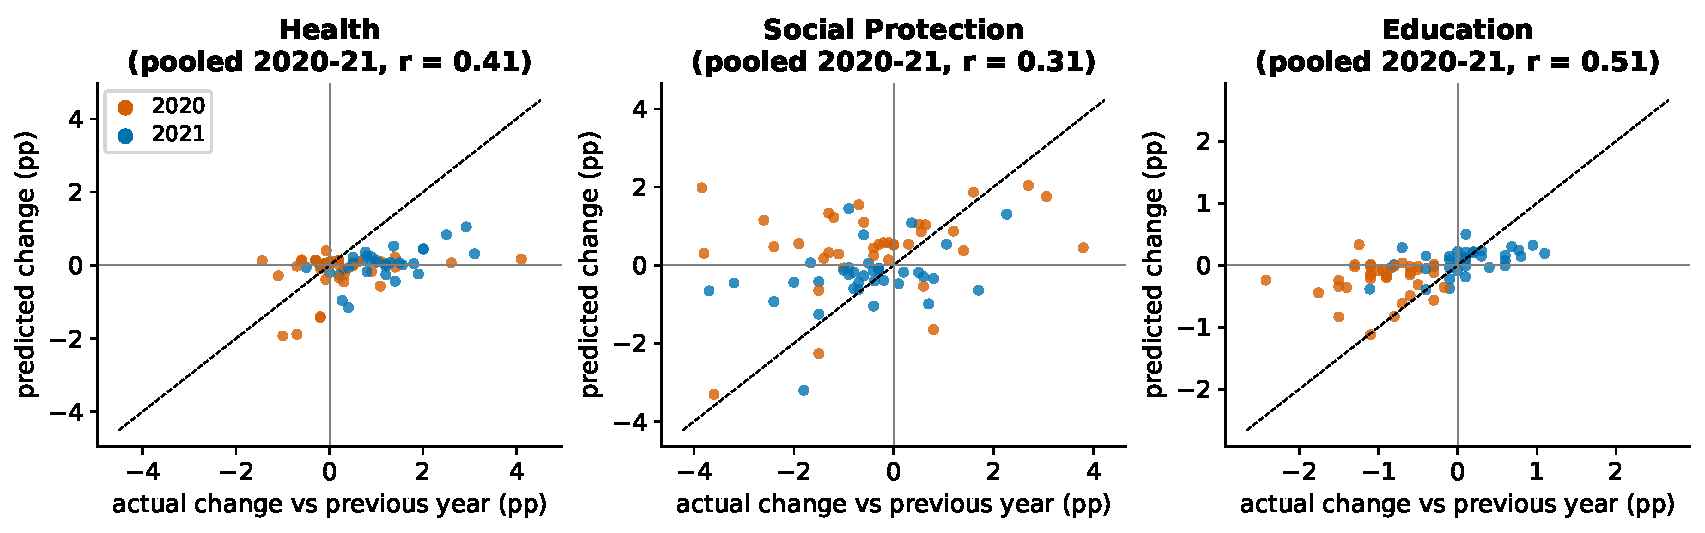
\includegraphics[width=\textwidth]{figures/fig10_covid_shift.pdf}
\caption{Predicted vs.\ observed one-year change in share, pooled 2020 and 2021 country-years (dashed line: perfect prediction); correlations are for the pooled points. The model captures the cross-country ranking only weakly and misses the aggregate shift.}\label{fig:covid}
\end{figure}}
